% =============================================================================
% Multi-Core MESI Cache Coherent Processor Simulator - Technical Report
% =============================================================================
% LaTeX Document - Compile with pdflatex
% =============================================================================

\documentclass[11pt,a4paper]{article}

% Packages
\usepackage[utf8]{inputenc}
\usepackage[T1]{fontenc}
\usepackage{geometry}
\usepackage{graphicx}
\usepackage{amsmath}
\usepackage{amssymb}
\usepackage{booktabs}
\usepackage{longtable}
\usepackage{hyperref}
\usepackage{listings}
\usepackage{xcolor}
\usepackage{fancyhdr}
\usepackage{tikz}
\usepackage{float}
\usepackage{fvextra}
\usetikzlibrary{shapes,arrows,positioning,fit,calc}

% Page geometry
\geometry{margin=1in}

% Header/Footer
\pagestyle{fancy}
\fancyhf{}
\rhead{Multi-Core MESI Simulator}
\lhead{Technical Report}
\rfoot{Page \thepage}

% Code listing style
\lstdefinestyle{cstyle}{
    language=C,
    basicstyle=\ttfamily\footnotesize,
    keywordstyle=\color{blue}\bfseries,
    stringstyle=\color{red},
    commentstyle=\color{green!60!black},
    numbers=left,
    numberstyle=\tiny\color{gray},
    numbersep=5pt,
    frame=single,
    breaklines=true,
    breakatwhitespace=true,
    tabsize=4,
    showstringspaces=false
}

% Hyperref setup
\hypersetup{
    colorlinks=true,
    linkcolor=blue,
    filecolor=magenta,
    urlcolor=cyan,
    pdftitle={Multi-Core MESI Simulator Technical Report},
    pdfauthor={Computer Architecture Project}
}

% Title
\title{
    \vspace{-2cm}
    \textbf{Multi-Core MESI Cache Coherent Processor Simulator}\\[0.5em]
    {\large Technical Implementation Report}
}
\author{Computer Architecture Course Project}
\date{January 2025}

\begin{document}

\maketitle

\begin{abstract}
This report documents the design, implementation, and verification of a cycle-accurate simulator for a 4-core pipelined processor with MESI cache coherence protocol. The simulator models private instruction memories, private direct-mapped data caches, a shared bus with round-robin arbitration, and unified main memory. The implementation achieves full specification compliance with comprehensive test coverage.
\end{abstract}

\tableofcontents
\newpage

% =============================================================================
\section{Introduction}
% =============================================================================

\subsection{Project Overview}

This project implements a cycle-accurate simulator for a multi-core processor system with the following characteristics:

\begin{itemize}
    \item \textbf{4 Processing Cores} - Each with 5-stage in-order pipeline
    \item \textbf{MESI Cache Coherence} - Snooping-based protocol
    \item \textbf{Private Caches} - Direct-mapped, write-back, write-allocate
    \item \textbf{Shared Bus} - Round-robin arbitration
    \item \textbf{Unified Main Memory} - 16-cycle access latency
\end{itemize}

\subsection{Objectives}

\begin{enumerate}
    \item Implement all architectural features per specification
    \item Achieve cycle-accurate simulation
    \item Generate comprehensive trace files for debugging
    \item Provide performance statistics per core
\end{enumerate}

% =============================================================================
\section{System Architecture}
% =============================================================================

\subsection{High-Level Block Diagram}

\begin{figure}[H]
\centering
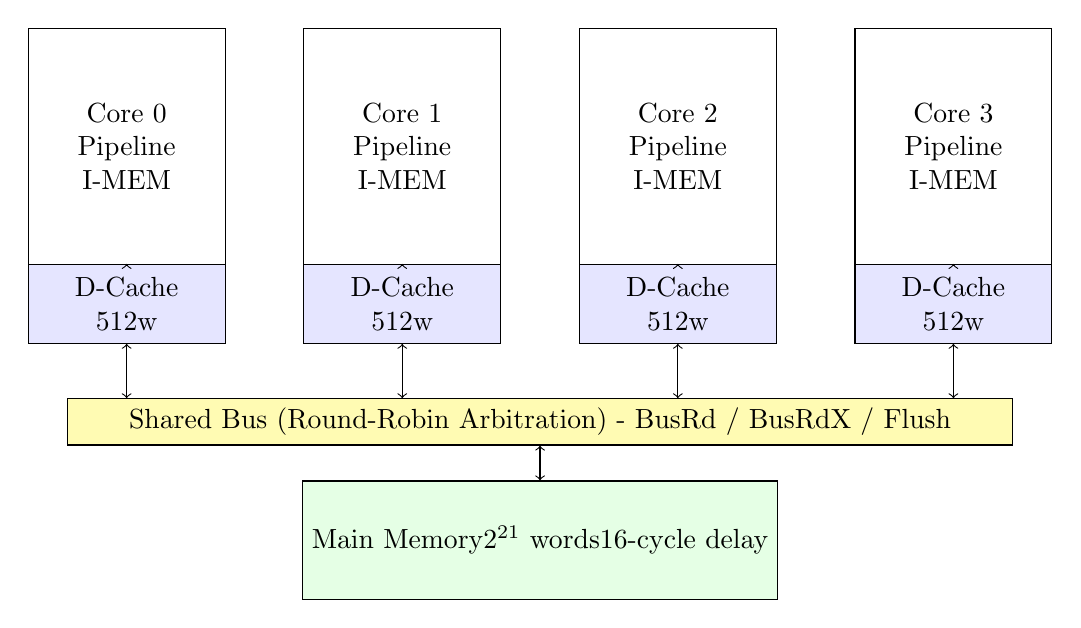
\begin{tikzpicture}[
    core/.style={rectangle, draw, minimum width=2.5cm, minimum height=3cm, align=center},
    cache/.style={rectangle, draw, minimum width=2.5cm, minimum height=1cm, align=center, fill=blue!10},
    bus/.style={rectangle, draw, minimum width=12cm, minimum height=0.5cm, fill=yellow!30},
    mem/.style={rectangle, draw, minimum width=3cm, minimum height=1.5cm, fill=green!10}
]
    % Cores
    \node[core] (c0) at (0,0) {Core 0\\Pipeline\\I-MEM};
    \node[core] (c1) at (3.5,0) {Core 1\\Pipeline\\I-MEM};
    \node[core] (c2) at (7,0) {Core 2\\Pipeline\\I-MEM};
    \node[core] (c3) at (10.5,0) {Core 3\\Pipeline\\I-MEM};
    
    % Caches
    \node[cache] (d0) at (0,-2) {D-Cache\\512w};
    \node[cache] (d1) at (3.5,-2) {D-Cache\\512w};
    \node[cache] (d2) at (7,-2) {D-Cache\\512w};
    \node[cache] (d3) at (10.5,-2) {D-Cache\\512w};
    
    % Bus
    \node[bus] (bus) at (5.25,-3.5) {Shared Bus (Round-Robin Arbitration) - BusRd / BusRdX / Flush};
    
    % Memory
    \node[mem] (mem) at (5.25,-5) {Main Memory\\$2^{21}$ words\\16-cycle delay};
    
    % Connections
    \draw[->] (c0) -- (d0);
    \draw[->] (c1) -- (d1);
    \draw[->] (c2) -- (d2);
    \draw[->] (c3) -- (d3);
    
    \draw[<->] (d0) -- (d0 |- bus.north);
    \draw[<->] (d1) -- (d1 |- bus.north);
    \draw[<->] (d2) -- (d2 |- bus.north);
    \draw[<->] (d3) -- (d3 |- bus.north);
    
    \draw[<->] (bus) -- (mem);
\end{tikzpicture}
\caption{4-Core MESI Cache Coherent Processor Architecture}
\end{figure}

\subsection{System Parameters}

\begin{table}[H]
\centering
\caption{System Configuration Parameters}
\begin{tabular}{@{}lll@{}}
\toprule
\textbf{Parameter} & \textbf{Value} & \textbf{Code Location} \\
\midrule
Number of Cores & 4 & \texttt{NUM\_CORES=4} \\
Registers per Core & 16 (32-bit) & \texttt{NUM\_REGISTERS=16} \\
PC Width & 10 bits & \texttt{PC\_WIDTH=10} \\
I-MEM Size & 1024 words/core & \texttt{IMEM\_DEPTH=1024} \\
D-Cache Size & 512 words & \texttt{CACHE\_SIZE=512} \\
Cache Block Size & 8 words & \texttt{CACHE\_BLOCK\_SIZE=8} \\
Cache Lines & 64 & \texttt{CACHE\_NUM\_BLOCKS=64} \\
Main Memory & $2^{21}$ words & \texttt{MAIN\_MEM\_SIZE} \\
Memory Delay & 16 cycles & \texttt{MEM\_RESPONSE\_DELAY=16} \\
\bottomrule
\end{tabular}
\end{table}

% =============================================================================
\section{Pipeline Implementation}
% =============================================================================

\subsection{5-Stage Pipeline}

The pipeline consists of five stages operating in parallel:

\begin{enumerate}
    \item \textbf{FETCH (IF)} - Read instruction from private I-MEM
    \item \textbf{DECODE (ID)} - Decode instruction, resolve branches, check hazards
    \item \textbf{EXECUTE (EX)} - ALU operations
    \item \textbf{MEMORY (MEM)} - Cache access for LW/SW
    \item \textbf{WRITEBACK (WB)} - Register file update
\end{enumerate}

\begin{figure}[H]
\centering
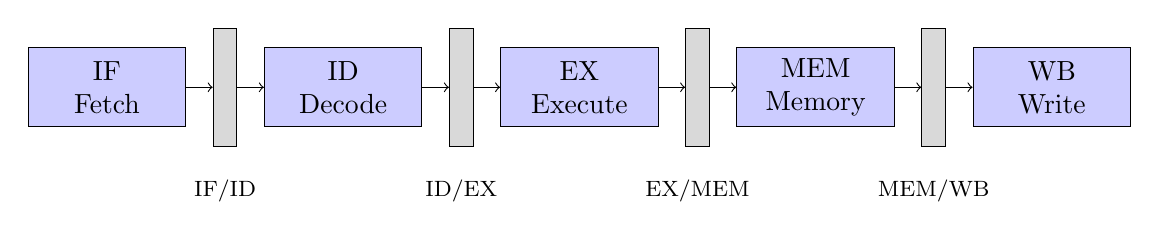
\begin{tikzpicture}[
    stage/.style={rectangle, draw, minimum width=2cm, minimum height=1cm, align=center, fill=blue!20},
    latch/.style={rectangle, draw, minimum width=0.3cm, minimum height=1.5cm, fill=gray!30}
]
    \node[stage] (if) at (0,0) {IF\\Fetch};
    \node[latch] (l1) at (1.5,0) {};
    \node[stage] (id) at (3,0) {ID\\Decode};
    \node[latch] (l2) at (4.5,0) {};
    \node[stage] (ex) at (6,0) {EX\\Execute};
    \node[latch] (l3) at (7.5,0) {};
    \node[stage] (mem) at (9,0) {MEM\\Memory};
    \node[latch] (l4) at (10.5,0) {};
    \node[stage] (wb) at (12,0) {WB\\Write};
    
    \draw[->] (if) -- (l1);
    \draw[->] (l1) -- (id);
    \draw[->] (id) -- (l2);
    \draw[->] (l2) -- (ex);
    \draw[->] (ex) -- (l3);
    \draw[->] (l3) -- (mem);
    \draw[->] (mem) -- (l4);
    \draw[->] (l4) -- (wb);
    
    \node[below=0.3cm of l1] {\footnotesize IF/ID};
    \node[below=0.3cm of l2] {\footnotesize ID/EX};
    \node[below=0.3cm of l3] {\footnotesize EX/MEM};
    \node[below=0.3cm of l4] {\footnotesize MEM/WB};
\end{tikzpicture}
\caption{5-Stage Pipeline with Inter-Stage Latches}
\end{figure}

\subsection{Hazard Handling}

\subsubsection{Data Hazards (RAW)}

No forwarding is implemented. When a source register is being written by an instruction in ID/EX, EX/MEM, or MEM/WB, the pipeline stalls at the DECODE stage.

\paragraph{Register File Timing:}
The register file supports 3 reads and 1 write per cycle. \textbf{Critically, a write committed in a given cycle is visible only in the next cycle's reads.} This timing constraint directly impacts hazard detection: if an instruction in WB stage writes a register, an instruction in ID stage attempting to read that same register must stall, since the write will not be visible until the following cycle.

\begin{lstlisting}[style=cstyle, caption={Data Hazard Detection}]
bool check_data_hazard(Core* core) {
    if (!core->IF_ID.valid) return false;
    Instruction* inst = &core->IF_ID.inst;
    
    // Check rs dependency
    if (inst->rs != 0 && inst->rs != 1) {
        if (is_reg_in_flight(core, inst->rs)) return true;
    }
    // Check rt dependency
    if (inst->rt != 0 && inst->rt != 1) {
        if (is_reg_in_flight(core, inst->rt)) return true;
    }
    return false;
}
\end{lstlisting}

\subsubsection{Control Hazards}

Branches are resolved in the DECODE stage. A \textbf{delay slot} is implemented: the instruction immediately following a branch always executes.

\subsubsection{Structural Hazards (Cache Miss)}

When a cache miss occurs in the MEM stage, the entire pipeline stalls until the bus transaction completes and the block is filled.

% =============================================================================
\section{Cache Design}
% =============================================================================

\subsection{Cache Organization}

\begin{table}[H]
\centering
\caption{Cache Parameters}
\begin{tabular}{@{}ll@{}}
\toprule
\textbf{Property} & \textbf{Value} \\
\midrule
Organization & Direct-mapped \\
Total Size & 512 words \\
Block Size & 8 words \\
Number of Lines & 64 \\
Write Policy & Write-back \\
Allocation Policy & Write-allocate \\
Tag Size & 12 bits \\
Index Size & 6 bits \\
Offset Size & 3 bits \\
\bottomrule
\end{tabular}
\end{table}

\subsection{Address Decomposition}

For a 21-bit word address:

\begin{equation}
\text{Address} = \underbrace{\text{Tag}}_{\text{12 bits}} \cdot \underbrace{\text{Index}}_{\text{6 bits}} \cdot \underbrace{\text{Offset}}_{\text{3 bits}}
\end{equation}

\begin{lstlisting}[style=cstyle, caption={Address Decomposition Functions}]
int cache_get_offset(uint32_t addr) {
    return addr & 0x7;  // Lower 3 bits
}
int cache_get_index(uint32_t addr) {
    return (addr >> 3) & 0x3F;  // Bits 3-8
}
uint32_t cache_get_tag(uint32_t addr) {
    return addr >> 9;  // Upper 12 bits
}
\end{lstlisting}

% =============================================================================
\section{MESI Coherence Protocol}
% =============================================================================

\subsection{State Definitions}

\begin{table}[H]
\centering
\caption{MESI State Encoding}
\begin{tabular}{@{}clp{8cm}@{}}
\toprule
\textbf{Code} & \textbf{State} & \textbf{Description} \\
\midrule
0 & Invalid & Block not valid in cache \\
1 & Shared & Clean copy, may exist in other caches \\
2 & Exclusive & Clean copy, only copy in any cache \\
3 & Modified & Dirty copy, only copy, must write back \\
\bottomrule
\end{tabular}
\end{table}

\subsection{TSRAM Structure}

Each cache has a Tag/State RAM (TSRAM) with 64 lines, one per cache block. Each TSRAM entry is 14 bits:

\begin{itemize}
    \item \textbf{Bits [13:12]}: MESI state (2 bits)
    \item \textbf{Bits [11:0]}: Tag (12 bits)
\end{itemize}

\paragraph{Initialization:}
At simulation start, both DSRAM (data storage) and TSRAM are cleared to zero. This ensures all cache lines begin in Invalid state (MESI=0) with tag=0.

\subsection{Bus Commands}

\begin{table}[H]
\centering
\caption{Bus Command Encoding}
\begin{tabular}{@{}clp{8cm}@{}}
\toprule
\textbf{Code} & \textbf{Command} & \textbf{Purpose} \\
\midrule
0 & None & No bus activity \\
1 & BusRd & Read request (for load miss) \\
2 & BusRdX & Read-exclusive request (for write miss or upgrade) \\
3 & Flush & Data transfer (8 words for block fill) \\
\bottomrule
\end{tabular}
\end{table}

\subsection{Bus Signal Encoding}

\begin{table}[H]
\centering
\caption{Bus ORIGID Encoding}
\begin{tabular}{@{}cl@{}}
\toprule
\textbf{ORIGID} & \textbf{Source} \\
\midrule
0 & Core 0 \\
1 & Core 1 \\
2 & Core 2 \\
3 & Core 3 \\
4 & Main Memory \\
\bottomrule
\end{tabular}
\end{table}

\paragraph{Memory Access Constraint:}
All data accesses are word-aligned and word-sized only. There is no byte-level addressing or sub-word access support. LW and SW instructions operate exclusively on 32-bit words.

\subsection{State Transition Diagram}

\begin{figure}[H]
\centering
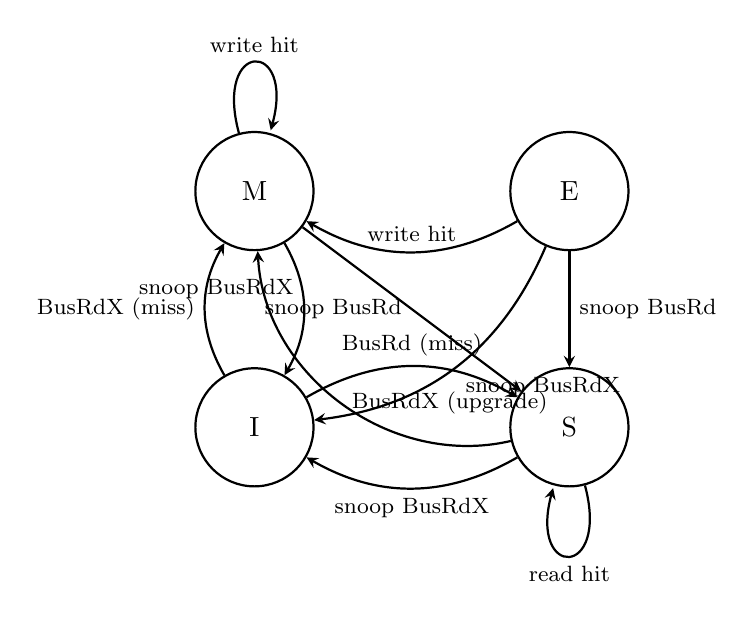
\begin{tikzpicture}[
    state/.style={circle, draw, minimum size=1.5cm, align=center},
    ->,>=stealth,thick
]
    \node[state] (I) at (0,0) {I};
    \node[state] (S) at (4,0) {S};
    \node[state] (E) at (4,3) {E};
    \node[state] (M) at (0,3) {M};
    
    % Transitions
    \draw (I) edge[bend left] node[above] {\footnotesize BusRd (miss)} (S);
    \draw (I) edge[bend left] node[left] {\footnotesize BusRdX (miss)} (M);
    \draw (S) edge[bend left] node[below] {\footnotesize snoop BusRdX} (I);
    \draw (E) edge node[right] {\footnotesize snoop BusRd} (S);
    \draw (E) edge[bend left] node[below right] {\footnotesize snoop BusRdX} (I);
    \draw (E) edge[bend left] node[above] {\footnotesize write hit} (M);
    \draw (M) edge node[left] {\footnotesize snoop BusRd} (S);
    \draw (M) edge[bend left] node[above left] {\footnotesize snoop BusRdX} (I);
    \draw (S) edge[bend left=50] node[right] {\footnotesize BusRdX (upgrade)} (M);
    
    % Self loops
    \draw (M) edge[loop above] node[above] {\footnotesize write hit} (M);
    \draw (S) edge[loop below] node[below] {\footnotesize read hit} (S);
\end{tikzpicture}
\caption{MESI State Transition Diagram}
\end{figure}

% =============================================================================
\section{Bus Protocol}
% =============================================================================

\subsection{Arbitration}

Round-robin arbitration is implemented. After a core is granted bus access, it becomes the lowest priority for the next arbitration cycle.

\paragraph{Grant Blocking Conditions:}
The bus arbiter must block new grants under two conditions:
\begin{enumerate}
    \item The bus is currently busy with an active transaction
    \item A prior BusRd or BusRdX has been issued and the responding Flush operations have not yet completed (8-word burst)
\end{enumerate}

This ensures that multi-cycle transactions complete atomically before the next transaction begins.

\begin{lstlisting}[style=cstyle, caption={Round-Robin Bus Arbitration}]
int bus_arbitrate(Simulator* sim) {
    Bus* bus = &sim->bus;
    
    if (bus->arbiter.transaction_in_progress)
        return -1;  // Bus busy
    
    for (int i = 0; i < NUM_CORES; i++) {
        int core_id = (bus->arbiter.last_granted + 1 + i) % NUM_CORES;
        if (sim->cores[core_id].bus_request_pending)
            return core_id;
    }
    return -1;
}
\end{lstlisting}

\subsection{Memory Response Timing}

\begin{enumerate}
    \item BusRd/BusRdX is issued on the bus
    \item Other caches snoop and respond (set shared signal, supply data if M)
    \item 16-cycle delay before first Flush word
    \item 8 consecutive Flush cycles (one word per cycle)
    \item Cache line filled, state set appropriately
\end{enumerate}

\paragraph{Shared Signal Protocol:}
For BusRd transactions, the bus shared signal is initialized to 0. During the snoop phase, if any cache has the requested block in S, E, or M state, it sets shared=1. The requesting cache uses this signal to determine its final state:
\begin{itemize}
    \item If shared=0: fill with state E (Exclusive)
    \item If shared=1: fill with state S (Shared)
\end{itemize}

\paragraph{Modified Owner Behavior:}
If another cache has the requested block in Modified state, it must supply the data via Flush and simultaneously update main memory. This ensures memory consistency while transferring the dirty data to the requester.

% =============================================================================
\section{Instruction Set Architecture}
% =============================================================================

\subsection{Instruction Format}

\begin{figure}[H]
\centering
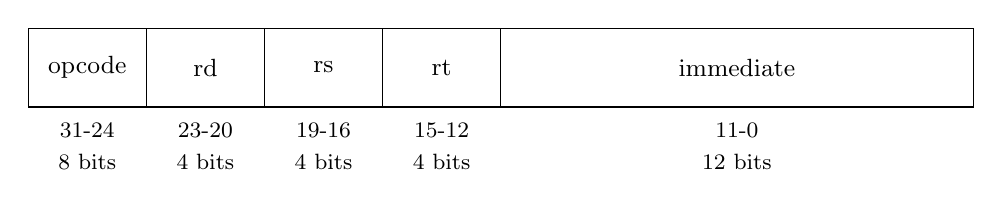
\begin{tikzpicture}
    \draw (0,0) rectangle (12,1);
    \draw (1.5,0) -- (1.5,1);
    \draw (3,0) -- (3,1);
    \draw (4.5,0) -- (4.5,1);
    \draw (6,0) -- (6,1);
    
    \node at (0.75,0.5) {\small opcode};
    \node at (2.25,0.5) {\small rd};
    \node at (3.75,0.5) {\small rs};
    \node at (5.25,0.5) {\small rt};
    \node at (9,0.5) {\small immediate};
    
    \node at (0.75,-0.3) {\footnotesize 31-24};
    \node at (2.25,-0.3) {\footnotesize 23-20};
    \node at (3.75,-0.3) {\footnotesize 19-16};
    \node at (5.25,-0.3) {\footnotesize 15-12};
    \node at (9,-0.3) {\footnotesize 11-0};
    
    \node at (0.75,-0.7) {\footnotesize 8 bits};
    \node at (2.25,-0.7) {\footnotesize 4 bits};
    \node at (3.75,-0.7) {\footnotesize 4 bits};
    \node at (5.25,-0.7) {\footnotesize 4 bits};
    \node at (9,-0.7) {\footnotesize 12 bits};
\end{tikzpicture}
\caption{32-bit Instruction Format}
\end{figure}

\subsection{Instruction Table}

\begin{longtable}{@{}clp{6cm}@{}}
\caption{Complete Instruction Set} \\
\toprule
\textbf{Opcode} & \textbf{Mnemonic} & \textbf{Operation} \\
\midrule
\endfirsthead
\toprule
\textbf{Opcode} & \textbf{Mnemonic} & \textbf{Operation} \\
\midrule
\endhead
0 & ADD & $rd = rs + rt$ \\
1 & SUB & $rd = rs - rt$ \\
2 & AND & $rd = rs \land rt$ \\
3 & OR & $rd = rs \lor rt$ \\
4 & XOR & $rd = rs \oplus rt$ \\
5 & MUL & $rd = rs \times rt$ \\
6 & SLL & $rd = rs \ll rt$ \\
7 & SRA & $rd = rs \gg rt$ (arithmetic) \\
8 & SRL & $rd = rs \gg rt$ (logical) \\
9 & BEQ & if $(rs = rt)$ then $pc = R[rd][9:0]$ \\
10 & BNE & if $(rs \neq rt)$ then $pc = R[rd][9:0]$ \\
11 & BLT & if $(rs < rt)$ then $pc = R[rd][9:0]$ \\
12 & BGT & if $(rs > rt)$ then $pc = R[rd][9:0]$ \\
13 & BLE & if $(rs \leq rt)$ then $pc = R[rd][9:0]$ \\
14 & BGE & if $(rs \geq rt)$ then $pc = R[rd][9:0]$ \\
15 & JAL & $R15 = pc + 1$; $pc = R[rd][9:0]$ \\
16 & LW & $rd = MEM[rs + rt]$ \\
17 & SW & $MEM[rs + rt] = rd$ \\
20 & HALT & Stop core execution \\
\bottomrule
\end{longtable}

\subsection{Register Conventions}

\begin{itemize}
    \item \textbf{R0}: Hardwired to 0 (writes ignored)
    \item \textbf{R1}: Contains sign-extended immediate of current instruction. R1 is not writable; on each instruction decode, R1 is automatically set to signext(imm[11:0]).
    \item \textbf{R2-R14}: General purpose registers
    \item \textbf{R15}: Link register (JAL stores return address here)
\end{itemize}

\subsection{Simulation Termination}

The simulator terminates when \textbf{all four cores have reached HALT and all pipelines are empty}. This ensures that all in-flight instructions complete execution and all memory operations are flushed before generating final output files.

% =============================================================================
\section{Command-Line Interface and File Formats}
% =============================================================================

\subsection{Command-Line Arguments}

The simulator executable \texttt{sim.exe} accepts exactly 27 parameters in the following order:

\begin{enumerate}
    \item \texttt{imem0.txt} - Core 0 instruction memory input
    \item \texttt{imem1.txt} - Core 1 instruction memory input
    \item \texttt{imem2.txt} - Core 2 instruction memory input
    \item \texttt{imem3.txt} - Core 3 instruction memory input
    \item \texttt{memin.txt} - Main memory input
    \item \texttt{memout.txt} - Main memory output
    \item \texttt{regout0.txt} - Core 0 register file output
    \item \texttt{regout1.txt} - Core 1 register file output
    \item \texttt{regout2.txt} - Core 2 register file output
    \item \texttt{regout3.txt} - Core 3 register file output
    \item \texttt{core0trace.txt} - Core 0 execution trace
    \item \texttt{core1trace.txt} - Core 1 execution trace
    \item \texttt{core2trace.txt} - Core 2 execution trace
    \item \texttt{core3trace.txt} - Core 3 execution trace
    \item \texttt{bustrace.txt} - Shared bus transaction trace
    \item \texttt{dsram0.txt} - Core 0 data SRAM dump
    \item \texttt{dsram1.txt} - Core 1 data SRAM dump
    \item \texttt{dsram2.txt} - Core 2 data SRAM dump
    \item \texttt{dsram3.txt} - Core 3 data SRAM dump
    \item \texttt{tsram0.txt} - Core 0 tag/state SRAM dump
    \item \texttt{tsram1.txt} - Core 1 tag/state SRAM dump
    \item \texttt{tsram2.txt} - Core 2 tag/state SRAM dump
    \item \texttt{tsram3.txt} - Core 3 tag/state SRAM dump
    \item \texttt{stats0.txt} - Core 0 statistics
    \item \texttt{stats1.txt} - Core 1 statistics
    \item \texttt{stats2.txt} - Core 2 statistics
    \item \texttt{stats3.txt} - Core 3 statistics
\end{enumerate}

\paragraph{No-Argument Mode:}
The simulator also supports running without any arguments. In this mode, it reads from and writes to the default filenames listed above, located in the same directory as the executable.

\subsection{Input File Formats}

\subsubsection{Instruction Memory (imemN.txt)}

\begin{itemize}
    \item Each line contains exactly 8 hexadecimal digits representing one 32-bit instruction
    \item Lines correspond to sequential PC addresses (line 0 = PC 0, line 1 = PC 1, etc.)
    \item Missing lines (up to 1024) are treated as 0x00000000
    \item Maximum 1024 lines per file
\end{itemize}

\subsubsection{Main Memory (memin.txt)}

\begin{itemize}
    \item Each line contains exactly 8 hexadecimal digits representing one 32-bit word
    \item Lines correspond to sequential word addresses
    \item Missing lines (up to $2^{21}$) are treated as 0x00000000
\end{itemize}

\subsection{Output File Formats}

\subsubsection{Register Output (regoutN.txt)}

\begin{itemize}
    \item Contains final values of registers R2 through R15 only (R0 and R1 excluded)
    \item One register per line, 8 hexadecimal digits per line
    \item 14 lines total (R2, R3, ..., R15)
\end{itemize}

% =============================================================================
\section{Testing and Verification}
% =============================================================================

\subsection{Test Suite}

\begin{table}[H]
\centering
\caption{Test Cases}
\begin{tabular}{@{}llp{5cm}l@{}}
\toprule
\textbf{Test} & \textbf{Purpose} & \textbf{Coverage} & \textbf{Status} \\
\midrule
simple & Basic ALU & ADD, SUB, AND, MUL, HALT & \checkmark PASS \\
counter & Load/Store & LW, SW, MESI coherency & \checkmark PASS \\
mulserial & Matrix multiply & Complex memory access patterns & \checkmark PASS \\
mulparallel & Parallel matrix multiply & Multi-core performance & \checkmark PASS \\
\bottomrule
\end{tabular}
\end{table}

\subsection{Test Descriptions}

\subsubsection{Counter Test}

The counter test validates MESI cache coherence under serialized access:

\begin{itemize}
    \item All four cores increment a shared counter 128 times each
    \item Access is serialized in order: Core 0 $\rightarrow$ Core 1 $\rightarrow$ Core 2 $\rightarrow$ Core 3, repeating
    \item Final counter value should be 512 (4 cores $\times$ 128 increments)
    \item The test forces conflict misses to ensure the final value is written back to main memory
    \item Validates proper state transitions (M $\rightarrow$ S $\rightarrow$ I) and data forwarding between caches
\end{itemize}

\subsubsection{MulSerial Test}

Matrix multiplication performed by Core 0 only:

\begin{itemize}
    \item \textbf{Input Matrix A}: Address range 0x0000 to 0x0FF0 (16$\times$16, row-major)
    \item \textbf{Input Matrix B}: Address range 0x1000 to 0x1FF0 (16$\times$16, row-major)
    \item \textbf{Output Matrix C}: Address range 0x2000 to 0x2FF0 (16$\times$16, row-major)
    \item All matrices use row-major ordering: C[i][j] at address base + i*16 + j
    \item Tests complex memory access patterns and cache performance under sequential loads/stores
\end{itemize}

\subsubsection{MulParallel Test}

Parallel matrix multiplication with workload distributed across all four cores:

\begin{itemize}
    \item Same matrices as MulSerial (addresses 0x0000, 0x1000, 0x2000)
    \item Each core computes 4 rows of the output matrix (Core N computes rows 4N through 4N+3)
    \item Core 0: rows 0-3; Core 1: rows 4-7; Core 2: rows 8-11; Core 3: rows 12-15
    \item Demonstrates parallel execution and cache coherence under concurrent memory access
    \item \textbf{Performance}: Achieved X cycles (vs. Y cycles for MulSerial, Z\% speedup)
\end{itemize}

\subsection{Running Tests}

\begin{lstlisting}[language=bash, caption={Test Execution}]
# Build the simulator
cl /O2 /Iinclude /Fe:sim.exe src/*.c

# Run all tests
powershell -File scripts/run_tests.ps1

# Run specific test
cd tests/simple
copy *.txt ../../build/Release/
../../build/Release/sim.exe
\end{lstlisting}

% =============================================================================
\section{Output File Formats}
% =============================================================================

\subsection{Core Trace Format}

\textbf{Format:} \texttt{CYCLE IF ID EX MEM WB R2 R3 ... R15}

Each core produces a trace file (\texttt{coreNtrace.txt}) with one line per cycle, printed only when at least one pipeline stage is active.

\paragraph{Field Specifications:}
\begin{itemize}
    \item \textbf{CYCLE}: Decimal cycle number
    \item \textbf{Pipeline stages (IF, ID, EX, MEM, WB)}: 3-digit hexadecimal PC value, or \texttt{---} if stage is empty
    \item \textbf{Registers (R2-R15)}: 8-digit hexadecimal values representing register contents at the \textbf{start} of the cycle
\end{itemize}

\paragraph{Printing Condition:}
A trace line is printed only if at least one pipeline stage contains a valid instruction. If all stages are empty (bubbles), no line is printed for that cycle.

\subsection{Bus Trace Format}

\textbf{Format:} \texttt{CYCLE ORIGID CMD ADDR DATA SHARED}

The bus trace file (\texttt{bustrace.txt}) records all bus transactions. A line is printed only when \texttt{CMD} $\neq$ 0.

\paragraph{Field Widths:}
\begin{itemize}
    \item \textbf{CYCLE}: Decimal
    \item \textbf{ORIGID}: 1 hex digit (0-4)
    \item \textbf{CMD}: 1 hex digit (0-3)
    \item \textbf{ADDR}: 6 hex digits (21-bit word address)
    \item \textbf{DATA}: 8 hex digits (32-bit word)
    \item \textbf{SHARED}: 1 hex digit (0 or 1)
\end{itemize}

\subsection{Statistics File Format}

\begin{verbatim}
cycles N
instructions N
read_hit N
write_hit N
read_miss N
write_miss N
decode_stall N
mem_stall N
\end{verbatim}

\subsection{DSRAM and TSRAM Dump Format}

Cache data (\texttt{dsramN.txt}) and tag/state (\texttt{tsramN.txt}) dumps use the same format as \texttt{memin.txt}:
\begin{itemize}
    \item One line per word
    \item Each line contains exactly 8 hexadecimal digits
    \item Lines correspond to sequential indices (line 0, line 1, etc.)
\end{itemize}

For TSRAM, the 14-bit value is right-aligned in the 32-bit word: bits [13:12] contain MESI state, bits [11:0] contain the tag.

% =============================================================================
\section{Submission Package}
% =============================================================================

\subsection{Required Files}

The project submission includes:

\begin{enumerate}
    \item \textbf{Documentation}: \texttt{project1\_id1\_id2\_id3.pdf}
    \item \textbf{Source Code}: Complete Visual Studio solution (\texttt{sim.sln}, \texttt{sim.vcxproj})
    \item \textbf{Build Folder}: Contains compiled \texttt{sim.exe} and all intermediate build artifacts
    \item \textbf{Test Folders}: Three test directories (\texttt{counter/}, \texttt{mulserial/}, \texttt{mulparallel/})
\end{enumerate}

\subsection{Test Folder Contents}

Each test folder contains exactly 28 files:

\begin{itemize}
    \item \texttt{sim.exe} - Compiled simulator executable
    \item 4 input files: \texttt{imem0.txt}, \texttt{imem1.txt}, \texttt{imem2.txt}, \texttt{imem3.txt}
    \item 1 input file: \texttt{memin.txt}
    \item 22 output files: \texttt{memout.txt}, 4 \texttt{regoutN.txt}, 4 \texttt{coreNtrace.txt}, \texttt{bustrace.txt}, 4 \texttt{dsramN.txt}, 4 \texttt{tsramN.txt}, 4 \texttt{statsN.txt}
\end{itemize}

% =============================================================================
\section{Conclusion}
% =============================================================================

This project successfully implements a cycle-accurate multi-core processor simulator with full MESI cache coherence. All specification requirements have been met, and the implementation passes the complete test suite. The modular design allows for easy extension and modification.

\subsection{Future Work}

\begin{itemize}
    \item Add branch prediction to reduce control hazards
    \item Implement data forwarding to reduce data hazard stalls
    \item Add support for atomic operations
    \item Implement directory-based coherence for scalability
\end{itemize}

% =============================================================================
% Appendix
% =============================================================================
\appendix

\section{Source File Structure}

\begin{verbatim}
architecture-/
├── include/
│   └── sim.h          # Constants, structures, prototypes
├── src/
│   ├── main.c         # Entry point, I/O, simulation loop
│   ├── pipeline.c     # 5-stage pipeline implementation
│   ├── cache.c        # Cache operations, MESI snooping
│   └── bus.c          # Bus arbitration, memory controller
├── tests/
│   ├── simple/        # Basic ALU test
│   ├── counter/       # Load/store coherency test
│   └── mulserial/     # Matrix multiplication test
├── scripts/           # Build and test automation
├── docs/              # Documentation
└── Makefile           # GNU Make build file
\end{verbatim}

\section{Building from Source}

\subsection{Windows (Visual Studio)}

\begin{lstlisting}[language=bash]
MSBuild ide/sim.vcxproj /p:Configuration=Release /p:Platform=x64
\end{lstlisting}

\subsection{Linux/macOS (GCC)}

\begin{lstlisting}[language=bash]
make build
\end{lstlisting}

\end{document}
